\documentclass[border=20pt]{standalone}
\usepackage{tikz}
\usepackage{amsmath}
\usetikzlibrary{calc,arrows.meta,angles,quotes}
\begin{document}
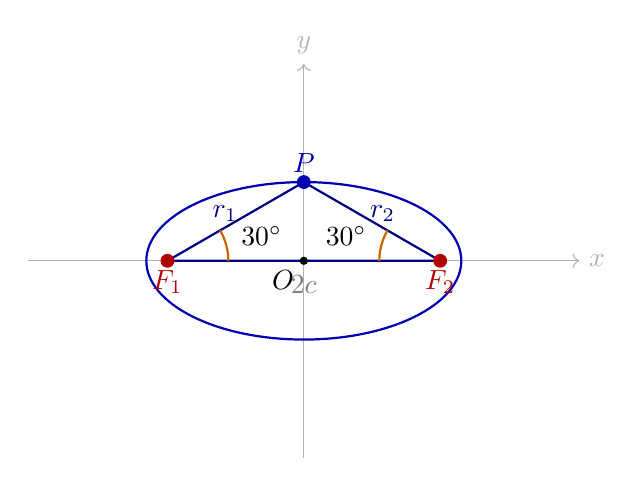
\begin{tikzpicture}[scale=1.0]
  % Axes
  \draw[->, gray!60, thin] (-3.5,0) -- (3.5,0) node[right] {$x$};
  \draw[->, gray!60, thin] (0,-2.5) -- (0,2.5) node[above] {$y$};

  % Ellipse: x^2/4 + y^2 = 1, a=2, b=1, c=√3≈1.732
  \draw[thick, blue!70!black] (0,0) ellipse (2 and 1);

  % Foci: F1(-√3,0), F2(√3,0)
  \coordinate (F1) at (-1.732, 0);
  \coordinate (F2) at (1.732, 0);
  \coordinate (O)  at (0,0);

  % P: symmetric (∠PF1F2=∠PF2F1=30°) → x_P=0, P=(0, b)=(0, 1)
  % ∠F1PF2 = 180° - 30° - 30° = 120°
  \coordinate (P) at (0, 1);

  % Triangle F1-P-F2
  \draw[thick, blue!50!black] (F1) -- (P) -- (F2) -- cycle;

  % Base angles at F1 and F2
  \draw pic["$30^\circ$", draw=orange!80!black, thick, angle eccentricity=1.6, angle radius=22] {angle=F2--F1--P};
  \draw pic["$30^\circ$", draw=orange!80!black, thick, angle eccentricity=1.6, angle radius=22] {angle=P--F2--F1};

  % Points
  \fill[red!70!black]  (F1) circle (2.5pt) node[below] {$F_1$};
  \fill[red!70!black]  (F2) circle (2.5pt) node[below] {$F_2$};
  \fill[blue!70!black] (P)  circle (2.5pt) node[above] {$P$};
  \fill[black]         (O)  circle (1.5pt) node[below left] {$O$};

  % Labels
  \node[blue!50!black] at (-1.0, 0.6) {$r_1$};
  \node[blue!50!black] at (1.0, 0.6)  {$r_2$};
  \node[gray] at (0, -0.3) {$2c$};
\end{tikzpicture}
\end{document}
